% Source of docs/architecture.png
% Build: pdflatex architecture.tex  then  pdftoppm -png -r 200 -singlefile architecture.pdf architecture
\documentclass[border=8pt]{standalone}
\usepackage{amsmath,amssymb,bm}
\usepackage{tikz}
\usetikzlibrary{arrows.meta,positioning,calc,decorations.pathmorphing}
\definecolor{ink}{HTML}{2B2D42}
\definecolor{lilac}{HTML}{CDB4DB}
\definecolor{lemon}{HTML}{FFF3B0}
\definecolor{peach}{HTML}{FFD6A5}
\definecolor{sky}{HTML}{BDE0FE}
\definecolor{mint}{HTML}{C7F9CC}
\definecolor{pinkD}{HTML}{D9779D}
\definecolor{mintD}{HTML}{5DAA78}
\begin{document}
\sffamily
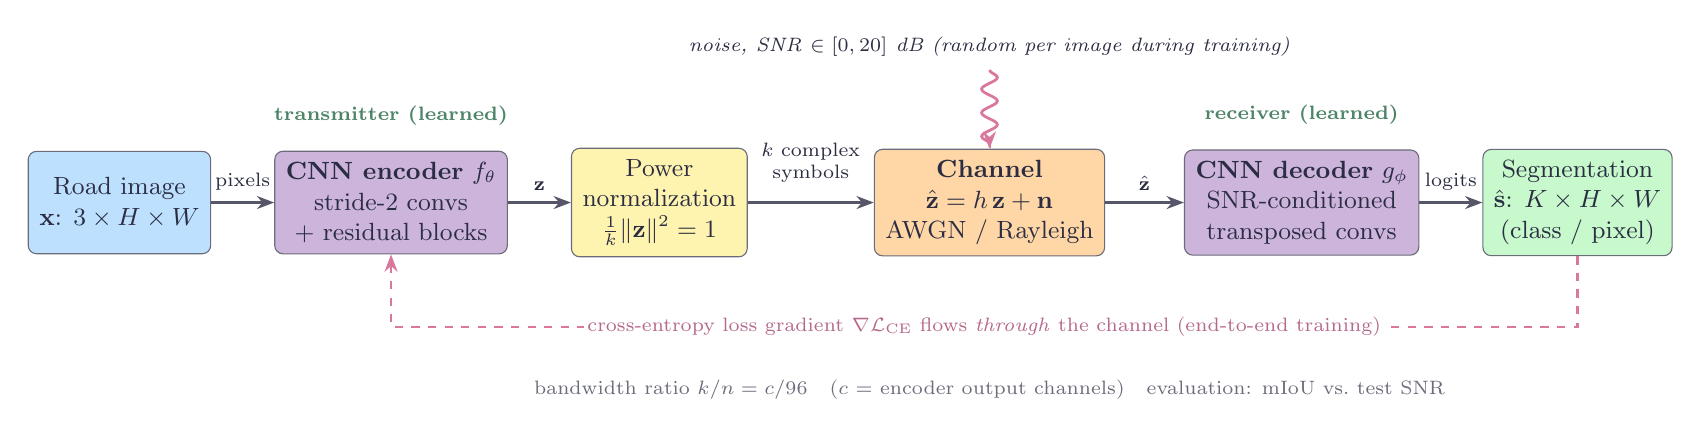
\begin{tikzpicture}[>={Stealth[length=2.2mm]}, node distance=7mm and 8mm, font=\small, text=ink,
  blk/.style={draw=ink!70, rounded corners=3pt, fill=#1, align=center, minimum height=1.3cm, inner sep=4pt},
  arr/.style={->, draw=ink!80, line width=0.8pt},
  lab/.style={font=\scriptsize, fill=white, inner sep=1.2pt, align=center}]
  \node[blk=sky, minimum width=1.9cm] (x) {Road image\\$\mathbf{x}$: $3\times H\times W$};
  \node[blk=lilac, right=of x, minimum width=2.3cm] (enc) {\textbf{CNN encoder} $f_\theta$\\stride-2 convs\\+ residual blocks};
  \node[blk=lemon, right=of enc, minimum width=1.9cm] (pn) {Power\\normalization\\$\tfrac1k\|\mathbf{z}\|^2=1$};
  \node[blk=peach, right=16mm of pn, minimum width=2.4cm] (ch) {\textbf{Channel}\\$\hat{\mathbf{z}} = h\,\mathbf{z} + \mathbf{n}$\\AWGN / Rayleigh};
  \node[blk=lilac, right=10mm of ch, minimum width=2.3cm] (dec) {\textbf{CNN decoder} $g_\phi$\\SNR-conditioned\\transposed convs};
  \node[blk=mint, right=of dec, minimum width=2.1cm] (s) {Segmentation\\$\hat{\mathbf{s}}$: $K\times H\times W$\\(class / pixel)};
  \draw[arr] (x) -- node[lab,above=1mm]{pixels} (enc);
  \draw[arr] (enc) -- node[lab,above=1mm]{$\mathbf{z}$} (pn);
  \draw[arr] (pn) -- node[lab,above=2mm]{$k$ complex\\symbols} (ch);
  \draw[arr] (ch) -- node[lab,above=1mm]{$\hat{\mathbf{z}}$} (dec);
  \draw[arr] (dec) -- node[lab,above=1mm]{logits} (s);
  \draw[decorate,decoration={snake,amplitude=1mm,segment length=3mm},draw=pinkD,line width=1pt,->]
       ($(ch.north)+(0,1.0)$) -- (ch.north);
  \node[font=\scriptsize\itshape, above=1.05cm of ch] {noise, SNR $\in[0,20]$ dB (random per image during training)};
  \draw[->, draw=pinkD, dashed, line width=0.9pt] (s.south) -- ++(0,-0.9) -| (enc.south);
  \node[lab, text=pinkD!80!ink] at ($(enc.south)!0.5!(s.south)+(0,-0.9)$)
       {cross-entropy loss gradient $\nabla\mathcal{L}_{\mathrm{CE}}$ flows \emph{through} the channel (end-to-end training)};
  \node[font=\scriptsize\bfseries, text=mintD!70!ink, above=2mm of enc] {transmitter (learned)};
  \node[font=\scriptsize\bfseries, text=mintD!70!ink, above=2mm of dec] {receiver (learned)};
  \node[font=\scriptsize, text=ink!70, below=1.45cm of ch, align=center] {bandwidth ratio $k/n = c/96$\quad($c$ = encoder output channels)\quad evaluation: mIoU vs.\ test SNR};
\end{tikzpicture}
\end{document}
